\documentclass{article}[11pt]

\usepackage[french]{babel}
\usepackage[utf8]{inputenc}
\usepackage{color}
\usepackage{graphicx}
\usepackage{amsmath}
\usepackage{hyperref}

\begin{document}

\Large

\title{Projet robotique autonome : \textbf{My Little Pony Ball catcher}}

\author{Victor Cheimanoff, Thibaud Cheippe, Yoan Mollard}

\maketitle

\normalsize

\tableofcontents

\begin{figure}[!htc]
	\begin{center}
		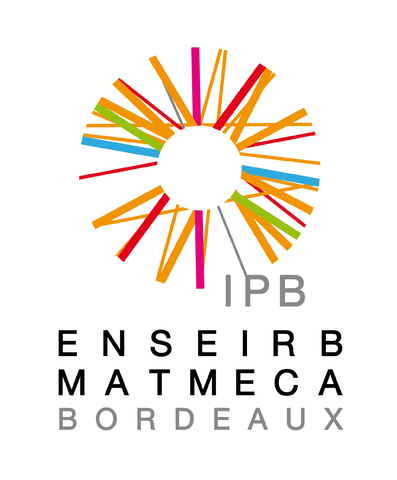
\includegraphics[scale=0.3]{images/logo_enseirb.png}
	\end{center}
\end{figure}

\newpage

\section{Introduction}

L'objet de ce projet est d'utiliser un bras robotique pour rattraper une balle qui lui serait lancée par un utilisateur. Le système utilise un équipement de motion tracking permettant de repérer la balle dans l'espace à l'aide de caméras. Une fois la trajectoire de la balle amorcée il calcule un point d'impact puis ordonne au bras de s'y positionner. \\

Bien que la main robotique soit capable de se fermer il semble important d'omettre ce détail dans un premier temps pour se consacrer sur l'obtention d'un impact entre la balle et le poignet. Ceci nottamment car orienter le bras dans une configuration où la balle peut rentrer au milieu des doigts ajout une difficulté supplémentaire. \\

Afin de conclure cette introduction nous présentons rapidement le matériel utilisé, à savoir le bras robotique et le système de capture Optitrack. L'ensemble de la scène est représenté en figure \ref{general}.

\subsection{Le bras robotique}

Le bras utilisé est un bras anthropomorphe à taille réelle conçu par Rhoban Project. Il dispose de sept servomoteurs Dynamixel immitant le bras humain. Il vient avec une suite logicielle .... TODO

\subsection{Le système de capture \og Motion tracking\fg}

Le système de capture utilisé est composé de trois caméras Optitrack VX1000. Equipées d'un éclairage infrarouge ces caméras, lorsqu'elles sont convenablement disposées autour d'une scène, permettent de localiser dans l'espace des boules réfléchissantes d'un centimètre de diamètre. Seuls les marqueurs réfléchissants fournis sont censés pouvoir être tracké par Optitrack. Cependant nous avons pensé à recouvrir notre balle de papier d'aluminium afin de substituer la balle aux marqueurs. \\

\begin{figure}[!htc]
	\begin{center}
		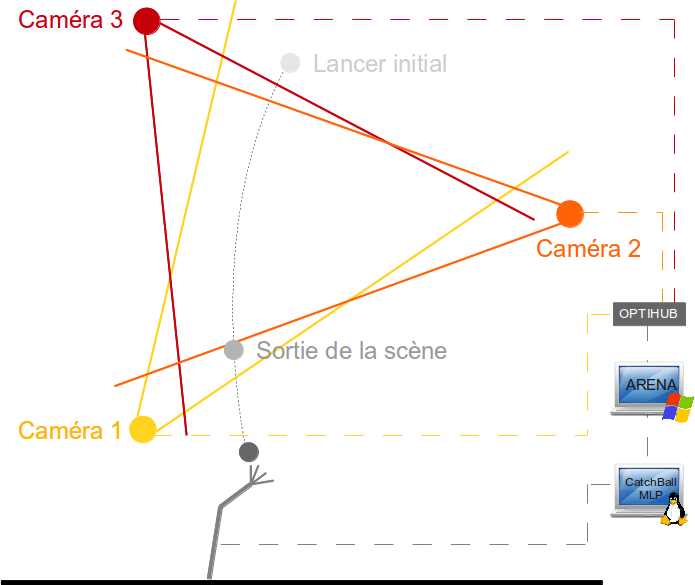
\includegraphics[scale=0.5]{images/general.png}
		\caption{Schéma de la scène : bras accompagné des trois caméras capturant le début de la trajectoire} 
		\label{general}
	\end{center}
\end{figure}

Nous avons décomposé le projet en trois parties distinctes :
\begin{itemize}
\item La mise en place du système de capture Optitrack de manière à obtenir les coordonnées x, y, z d'un point de l'espace
\item L'obtention du modèle géométrique inverse du robot, le calcul de la trajectoire de la balle et la planification du point d'impact
\item La réalisation d'une représentation OpenGL de la scène pour visualiser 
\end{itemize}

\section{Exportation des coordonnées d'un point avec Optitrack}

Cette partie est un tutoriel de mise en route rapide du système de capture, principalement à destination des futurs utilisateurs ou repreneurs du projet. Le fabriquant du système documente peu ses produits mais les tutoriels sont plutôt utiles \cite{naturalpoint_tutoriels}. \\

La première étape consiste à disposer les caméras autour de la scène. Six caméras sont fournies dans le pack, mais nous avons commencé par en monter seulement trois sur trépied. Selon la qualité des résultats obtenus il est possible d'ajouter des trois autres à mi-hauteur sur les trépieds pour augmenter la précision des coordonnées obtenus. \\

Les trois (ou les six) caméras sont connectées à un hub USB (Optihub) lui-même connecté à un PC sur lequel est installé le logiciel Arena. Il est important de disposer les caméras plutôt vers le début de la trajectoire de la balle, car c'est ici qu'il nous reste suffisamment de temps pour effectuer les calculs et surtout positionner le bras robot à la position calculée. \\

\subsection{Calibration des caméras}

La première étape consiste à calibrer les caméras entre elles. En démarrant l'utilitaire de calibration d'Arena on commence par jouer sur les paramètres ainsi que sur l'orientation des caméras. Selon nos essais, il est préférable d'éviter que les caméras se voient les-unes-les-autres et de choisir une intensité faible pour les LEDs infrarouge : une trop forte intensité augmente le nombre de parasites. Avant de continuer il faut s'assurer qu'aucun point parasite n'est détecté par l'une des caméras en l'abscence de marqueur dans la scène. Les parasites peuvent être des objets réfléchissants ou brillants (fenêtre, lumière, métal ...). Afin de comprendre d'où proviennent les parasites il est utile d'afficher les images noir et blanc renvoyées par les caméras (clic droit sur une frame > Grayscale image). Avant de commencer la calibration aucun parasite ne doit apparaître en l'absence de marqueur et un marqueur placé dans la scène doit être reconnu par les trois caméras. \\

L'étape de calibration peut ensuite commencer. Il s'agit de déplacer trois marqueurs au bout d'une baguette Optiwand pour couvrir au maximum le volume de la scène dans un maximum d'orientations possibles. Toutes les caméras doivent visualiser les marqueurs pour que les points puissent participer à la calibration. A l'issue du processus de calcul Arena est capable de disposer les caméras dans l'espace les unes par rapport aux autres sur une carte. \\

Note : la licence Arena a été enregistrée pour la caméra 179282. Cette caméra doit donc impérativement être branchée pour démarrer Arena.

\subsection{Constitution d'un Corps Rigide}

Pouet ?

\subsection{Exportation des coordonnées}

Arena embarque un serveur diffusant les coordonnées du corps rigide. Un client récupérant ces coordonnées existe déjà pour Windows, nous l'avons adapté pour qu'il puisse fonctionner sous Linux et pour l'intégrer à notre Ball catcher. 

\section{Modélisation et prédiction d'impact}
Victor ...

\section{Représentation 3D de la scène, du bras, de la balle et de sa trajectoire}

Nous avons ajouté au projet un visualisateur 3D pour représenter la scène. L'intérêt est de pouvoir remplacer le bras matériel par un bras simulé et d'afficher les résultats théoriques. Le minimum, et de loin le plus important est de représenter le système de coordonnées de la scène (défini par le Calibration Square), la trajectoire prévue et affinée à chaque instant, et le point d'impact calculé. \\

Les trois fichiers \textit{main}, \textit{window} et \textit{glwidget} s'occupent du fonctionnement global de l'application, de la fenêtre, et du composant OpenGL. La scène est dessinée dans $GLWidget::paintGL()$, méthode appelée à chaque rafraichissement de l'image. Les éléments de la scène (balle, sol, mur, robot ...) sont déclarés dans l'en-tête de GLWidget et dessinés dans cette méthode $paintGL()$. Les éléments affichables sont :\\

\begin{itemize}
\item \textit{CoordinateSystem} : Le visualisateur dispose d'une classe \textit{CoordinateSystem} qui représente le système de coordonnées de la scène. Il est déplacé en fonction du système de coordonnées OpenGL pour correspondre à celui réellement utilisé dans la scène.
\item \textit{Ball} : 
\item 
\end{itemize}



\section{Conclusion}


\begin{thebibliography}{}
  \bibitem{naturalpoint_tutoriels}
  Tutoriels NaturalPoint Optitrack \\
  \url{http://www.naturalpoint.com/optitrack/products/arena/tutorials.html}

\end{thebibliography} 

\end{document}
